% RLC main.tex Version 2024.2

\documentclass[10pt]{article} % For LaTeX2e
\usepackage{rlc}
\usepackage{amsmath}

% If accepted, instead use the following line for the camera-ready submission:
%\usepackage[accepted]{rlc}
% To de-anonymize and remove mentions to RLC (for example, for posting to preprint servers), instead use the following:
% \usepackage[preprint]{rlc}

%%%%%%%%%%%%%%%%%%%%%%%%%%%%%%%%%%%%%%%%%%%%%%%%%%%%%%%%%%%%%%%%
%% Recommended (but not required) packages
%%%%%%%%%%%%%%%%%%%%%%%%%%%%%%%%%%%%%%%%%%%%%%%%%%%%%%%%%%%%%%%%
\usepackage{amssymb}            % Defines common symbols like \mathbb R
\usepackage{mathtools}          % Extends amsmath, providing common math tools
\usepackage{mathrsfs}           % Enables \mathscr, which can work in cases that \mathcal does not
\mathtoolsset{showonlyrefs}     % Only number equations that are referenced (optional)
\usepackage{graphicx}           % For including images
\usepackage{subcaption}         % Allows for the use of subfigures and subcaptions
\usepackage[space]{grffile}     % For spaces in image names
\usepackage{url}                % For displaying urls

%%%%%%%%%%%%%%%%%%%%%%%%%%%%%%%%%%%%%%%%%%%%%%%%%%%%%%%%%%%%%%%%
%% Title Page Specification
%%%%%%%%%%%%%%%%%%%%%%%%%%%%%%%%%%%%%%%%%%%%%%%%%%%%%%%%%%%%%%%%
\title{Models of the thesis}

% Authors must not appear in the submitted version. They should be hidden
% as long as the tmlr package is used without the [accepted] or [preprint] options.
% Non-anonymous submissions will be rejected without review.

\author{Philip S. Thomas  \\
    pthomas@cs.umass.edu \\
    College of Information and Computer Sciences\\
    University of Massachusetts
    \And
    Glen Berseth \\
    glen.berseth@mila.quebec\\
    Mila, Universit\'e de Montr\'eal \\
    CIFAR Canada AI Chair}

% The \author macro works with any number of authors. Use \AND 
% to\ separate the names and addresses of multiple authors.

%%%%%%%%%%%%%%%%%%%%%%%%%%%%%%%%%%%%%%%%%%%%%%%%%%%%%%%%%%%%%%%%
%% Begin document, create title and abstract
%%%%%%%%%%%%%%%%%%%%%%%%%%%%%%%%%%%%%%%%%%%%%%%%%%%%%%%%%%%%%%%%
\begin{document}
    \bibliographystyle{plain}  % Scegli uno stile adatto
    
    \section{Information about the dataset and pre-processing}
    The dataset used is AgrImOnIA V 3.0.0 \cite{lmwebsite}. The considered station is Bertonico (IDstation 1266).
    \\The variables used for the regressions are weather (WE) and emissions (EM). 
    \\For the pre-processing part it was used a the standardization and is described in the equation \ref{eq:normalization}.

    \begin{equation}
        X_{standardized} = \frac{X-\mu}{\sigma}
        \label{eq:normalization} 
    \end{equation}

    \\This process improves the interpretability and the training convergence. Furthermore it reduces the risk of outliers.
    \\Following this phase it was created the correlation matrix for removing the terms that are correlated and they are: $EM\_nh3\_agr\_waste\_burn$, $EM\_nox\_traffic$, $EM\_nox\_sum$, $EM\_so2\_sum$, $WE\_temp\_2m$, $WE\_wind\_speed\_10m\_mean$, $WE\_blh\_layer\_max$, $WE\_blh\_layer\_min$, $WE\_tot\_precipitation$ and $WE\_precipitation\_t$.
    \section{Lasso Regression Model}
    \subsection{Classical formulation of the problem}
    The cost function associated to this model is similar to the Ridge's one except for the regularization term.
    \\The cost function \cite{james2013chapter6-2-2} associated to the lasso regression is \ref{eq:lasso}.
    \\As is evident from the two equations, the regularization term in Lasso is based on \( \lambda \sum_{j=1}^p|\beta_j| \), where \( \lambda \) is the regularization parameter and \( p \) is the number of features. This term involves the absolute values of the regression coefficients (\( \beta_j \)), promoting sparsity in the model by encouraging some coefficients to be exactly zero. In contrast, the regularization term in Ridge is \( \lambda \sum_{j=1}^p \beta_j^2 \), which includes the squared values of the coefficients. The squared term tends to shrink the coefficients towards zero but rarely makes them exactly zero. As a result, Ridge regression may include all features with reduced weights, but none are completely excluded. The choice between Lasso and Ridge regularization depends on the desired characteristics of the model, with Lasso being effective for feature selection when dealing with high-dimensional datasets and Ridge providing more stability when multicollinearity is a concern.

    \begin{equation}
    \min \left\{ \sum_{i=1}^n \left( y_i - \beta_0 - \sum_{j=1}^p \beta_j x_{ij} \right)^2 + \lambda \sum_{j=1}^p \left| \beta_j \right| \right\} = \min \left\{ \text{RSS} + \lambda \sum_{j=1}^p \left| \beta_j \right| \right\}
         \label{eq:lasso} 
    \end{equation}
    where:
    \begin{itemize}
        \item $n$ is the total number of observations in the dataset,
        \item $y_i$ is the value of the dependent variable for observation $i$,
        \item $\beta_0$ is the intercept term,
        \item $p$ is the number of independent variables in the model,
        \item $x_{ij}$ represents the value of predictor $j$ for observation $i$,
        \item $\beta_j$ are the coefficients associated with the independent variables,
    \end{itemize}
    \subsection{Implementation}

    Also in this model it was used cv.glment as library but in this case for making a lasso regression the value of $\alpha$ should be equal to 1.

    \subsection{Results}
    The best value for the parameter $\lambda$ obtained for the process is $1.082 \cdot 10^{-05}$. This value is crucial as it regulates the regularization in the model, influencing the balance between fitting the data and the model's complexity. A higher $\lambda$ tends to favor simpler models at the expense of a tighter fit to the training data.
    
    The associated values of the parameters are as follows:
    
    \begin{table}[h]
    \centering
    \begin{tabular}{lll}
    \toprule
    Variable & Coefficient & Standard Deviation \\
    \midrule
    $$EM\_nh3\_agr\_waste\_burn$$ & 0.1896 & 0.3535 \\
    $$EM\_nox\_traffic$$ & 0.0896 & 0.2323 \\
    $$EM\_nox\_sum$$ & 0.1273 & 0.2331 \\
    $$EM\_so2\_sum$$ & -0.2378 & 0.3000 \\
    $$WE\_temp\_2m$$ & 0.1104 & 0.2326 \\
    $$WE\_wind\_speed\_10m\_mean$$ & 0.1742 & 0.1261 \\
    $$WE\_blh\_layer\_max$$ & -0.1400 & 0.1431 \\
    $$WE\_blh\_layer\_min$$ & -0.1391 & 0.0762 \\
    $$WE\_tot\_precipitation$$ & -0.1847 & 0.1124 \\
    $$WE\_precipitation\_t$$ & -0.1389 & 0.0942 \\
    $$Intercept$$ & -0.1560 & NA \\
    \bottomrule
    \end{tabular}
    \caption{Coefficients with Standard Deviations of the polynomial regression}
    \label{tab:coefficients}
    \end{table}

    Now, let's examine the coefficients associated with these parameters. For instance, $EM\_nh3\_agr\_waste\_burn$ has a positive coefficient of 0.2192, indicating that an increase in this variable is associated with an increase in the response variable. On the other hand, some coefficients are negative, suggesting that an increase in those variables is associated with a decrease in the response variable.

    The Polynomial Regression model, characterized by its flexibility in capturing non-linear relationships, exhibits a commendable performance with a Root Mean Squared Error ($RMSE$) of $0.087$. This low RMSE value indicates a strong fit to the data, suggesting that the polynomial features effectively model the underlying complexity in the dataset. However, it's important to strike a balance in polynomial degree to avoid overfitting. Fine-tuning the model's complexity is crucial, as excessively high-degree polynomials may lead to capturing noise instead of true patterns. Nonetheless, when appropriately configured, Polynomial Regression proves to be a powerful tool for capturing intricate relationships in the data.
    
    \subsection{Residual analysis}

    The Lasso Regression model, incorporating a regularization technique, achieves a Root Mean Squared Error ($RMSE$) of $0.1036$. This low $RMSE$ value signifies a robust fit to the data, demonstrating that the model's predictions closely align with the actual values. Lasso Regression, by utilizing a sparsity-inducing penalty, not only aids in feature selection but also contributes to the prevention of overfitting, enhancing the model's generalization ability on new, unseen data.
    
    Additionally, further statistics on the residuals of the model are provided:
    
    - \textbf{Skewness}: Measures the asymmetry of the distribution of residuals. A value of 1.144 suggests a slight positive skewness.
    
    - \textbf{Mean}: The mean of the residuals is 0.02, indicating that, on average, the model does not exhibit systematic bias.
    
    - \textbf{Standard Deviation}: The standard deviation of the residuals is 0.1038, representing the dispersion of residuals around their mean.
    
    - \textbf{Kurtosis}: Measures the "heaviness of the tails" of the distribution of residuals. A value of 3.17 suggests heavier tails compared to a normal distribution.
    
    These statistics collectively provide insights into both the parameter values and the overall performance of the model.
    
     \begin{figure}[h]
        \centering
        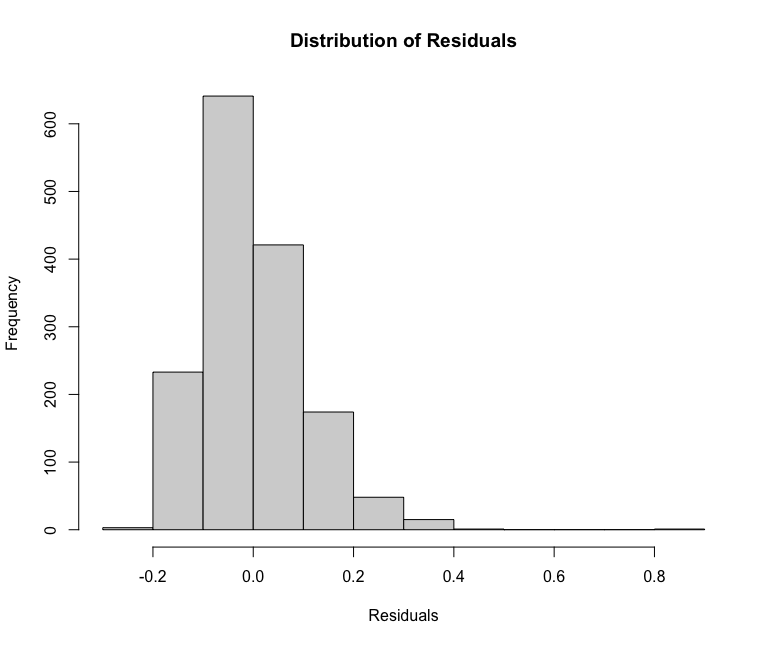
\includegraphics[scale=0.45]{Assets/distribution_ridge.png}
        \caption{Error distribution for the ridge regression}
        \label{fig:enter-label}
    \end{figure}
    \begin{figure}[h]
        \centering
        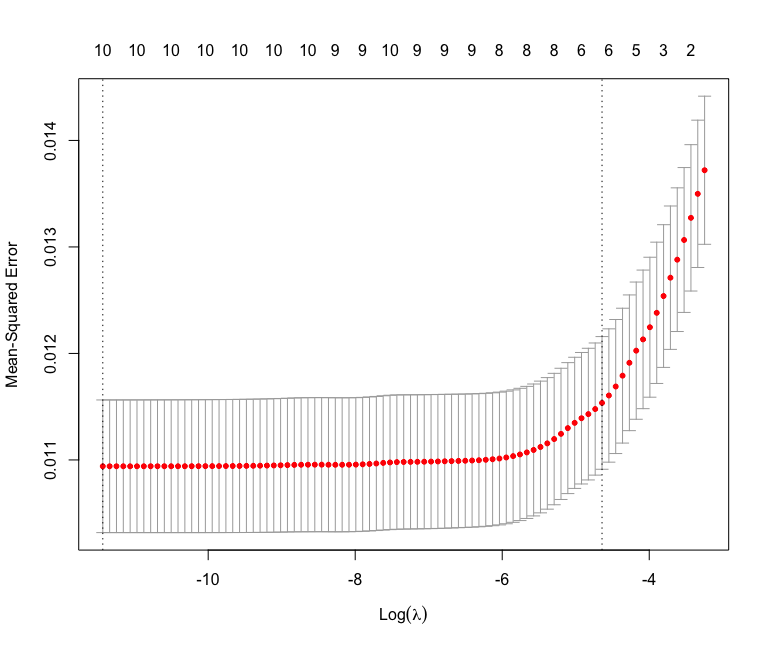
\includegraphics[scale=0.5]{Assets/Lasso.png}
        \caption{Lasso regression $Log(\lambda)$ graph}
        \label{fig:enter-label}
    \end{figure}

    \begin{figure}[h]
        \centering
        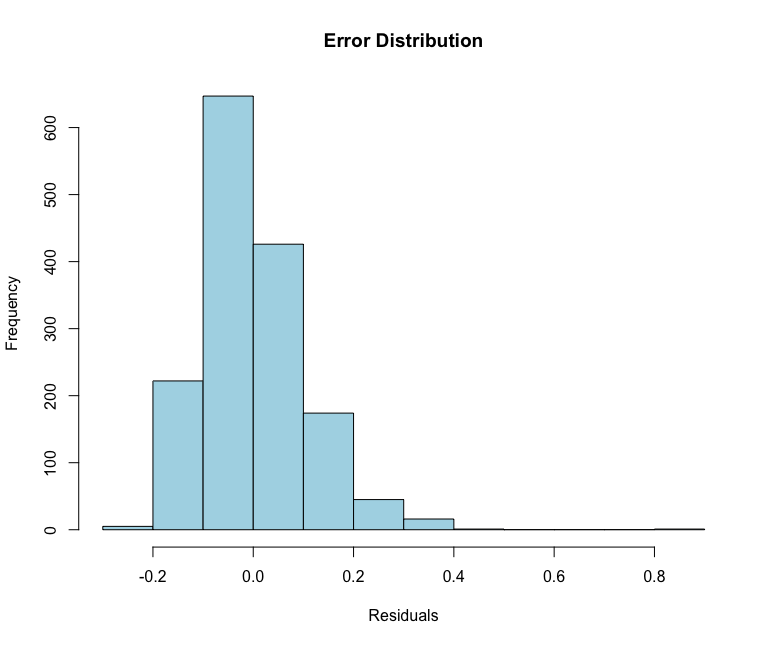
\includegraphics[scale=0.45]{Assets/Errors lasso.png}
        \caption{Residuals distribution for Lasso regression}
        \label{fig:enter-label}
    \end{figure}
    \newpage
    \subsubsection{Autocorrelatio of the residuals}
    Autocorrelation of residuals is a measure of the correlation between consecutive residuals in a time series or, more generally, in a model's residuals. In the context of a Lasso (Least Absolute Shrinkage and Selection Operator) model, autocorrelation in residuals indicates that there might be patterns or dependencies left unexplained by the model. An autocorrelation coefficient of 0.554663 suggests a moderate positive correlation between successive residuals. This autocorrelation implies that there might be temporal dependencies or trends in the data that are not captured by the Lasso model. Detecting and addressing autocorrelation is essential for ensuring the model's reliability and making accurate predictions. Techniques such as including lagged variables or using time series models may help address autocorrelation in the residuals of a Lasso model.

    \section{Ridge regression}
    \subsection{Classical formulation of the problem}
    The ridge regression cost function \cite{james2013chapter6-2-1} is described in the equation \ref{eq:ridge}.

    \begin{equation}
        \min \left\{\sum_{i=1}^n\left(y_i-\beta_0-\sum_{j=1}^p \beta_j x_{i j}\right)^2+\lambda \sum_{j=1}^p \beta_j^2 \right\}= \left\{\operatorname{RSS}+\lambda \sum_{j=1}^p \beta_j^2 \right\}
        \label{eq:ridge} 
    \end{equation}

    Where:
     \begin{itemize}
        \item $n$ is the total number of observations in the dataset,
        \item $y_i$ is the value of the dependent variable for observation $i$,
        \item $\beta_0$ is the intercept term,
        \item $p$ is the number of independent variables in the model,
        \item $x_{ij}$ represents the value of predictor $j$ for observation $i$,
        \item $\beta_j$ are the coefficients associated with the independent variables,
        \item $\lambda$ is the regularization term,
    \end{itemize}

    \subsection{Implementation}
    The package used in R is cv.glmnet \cite{glmnetwebsite}. This package makes cross validation with a $\lambda$ which changes at each iteration of the cross-validation and the plot of the process. It is necessary to keep $\alpha$ equal to 0. 
    The result is described in the figure \ref{fig:ridge-results}.

    \subsection{Results}
    The best $\lambda$ associated at the process of the crossvalidation is 0.00389.
  The following are the coefficients estimated by Ridge Regression for various variables:

    \begin{table}[htbp]
    \centering
    \begin{tabular}{lcc}
    \toprule
    Variable & Coefficient (Ridge) & Standard Deviation \\
    \midrule
    EM\_nh3\_agr\_waste\_burn & 0.2192 & 0.3535 \\
    EM\_nox\_traffic & 0.0302 & 0.2323 \\
    EM\_nox\_sum & -0.0105 & 0.2331 \\
    EM\_so2\_sum & -0.0419 & 0.3000 \\
    WE\_temp\_2m & 0.0313 & 0.2326 \\
    WE\_wind\_speed\_10m\_mean & 0.1400 & 0.1261 \\
    WE\_blh\_layer\_max & -0.1417 & 0.1431 \\
    WE\_blh\_layer\_min & -0.1279 & 0.0762 \\
    WE\_tot\_precipitation & -0.1818 & 0.1124 \\
    WE\_precipitation\_t & -0.1362 & 0.0942 \\
    NA & -0.1535 & NA \\
    \bottomrule
    \end{tabular}
    \caption{Coefficients and Standard Deviations for Ridge Model}
    \label{tab:ridge_coefficients}
    \end{table}
    
    These coefficients indicate the effect of the respective variables on the response variable, with positive values indicative of an increase in the response and negative values indicating a decrease.

    The Ridge Regression model with a regularization parameter produces a Root Mean Squared Error ($RMSE$) of $0.1038$, indicating a strong fit to the data. This low $RMSE$ value suggests that the model's predictions closely align with the actual values. The regularization in Ridge Regression helps control overfitting, enhancing the model's generalization performance on new, unseen data.
    
    It is noteworthy that the errors associated with the coefficients exhibit a Gaussian distribution, characterized by a mean of 0, a standard deviation of 0.1038, skewness of 1.1444, and a kurtosis of 3.1743. This observation indicates that the ridge regression model is effectively capturing the variability present in the data. The Gaussian nature of these errors is a positive indication of the model's goodness of fit.

    \subsubsection{Residual analysis}
    The Gaussian distribution of errors implies that the residuals of the model follow a normal distribution, with a mean of 0, reflecting the absence of systematic bias. The standard deviation of 0.1038 signifies the dispersion of residuals around their mean, offering insights into the consistency of the model's predictions. The skewness of 1.1444 suggests a slight positive skewness, indicating a departure from perfect symmetry in the distribution of residuals. Furthermore, the kurtosis of 3.1743 highlights that the tails of the distribution are heavier than those of a normal distribution.
    
    The presence of Gaussian errors reinforces the reliability of the ridge regression model, emphasizing its capability to not only capture the central tendency of the data but also to provide a reasonable representation of the spread and shape of the residuals. The normality in the errors suggests a well-fitted model that adequately accounts for the underlying variability in the observed data, contributing to the model's overall effectiveness in explaining the relationships among the variables.


    \begin{figure}[h]
        \centering
        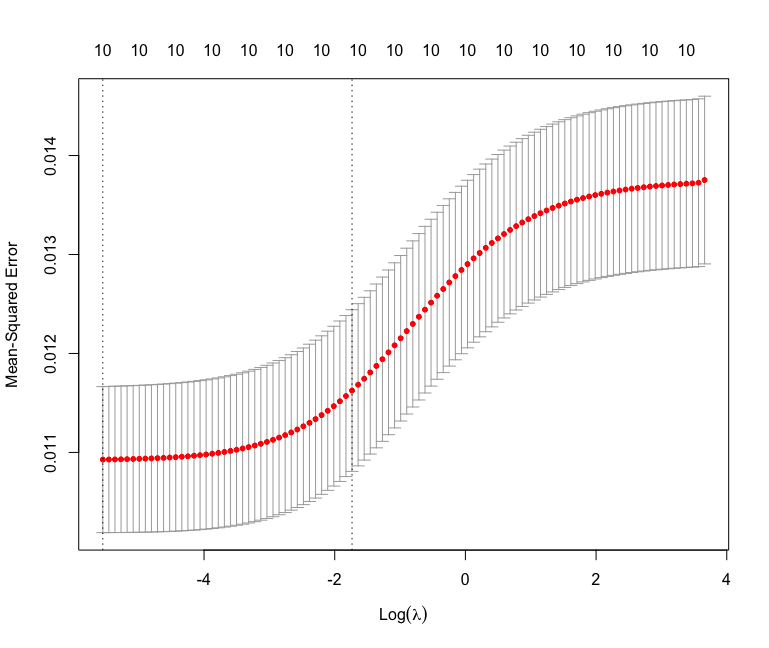
\includegraphics[scale=0.45]{Assets/Ridge.png}
        \caption{Ridge regression $Log(\lambda)$ graph}
        \label{fig:ridge-results}
    \end{figure}

    \begin{figure}
        \centering
        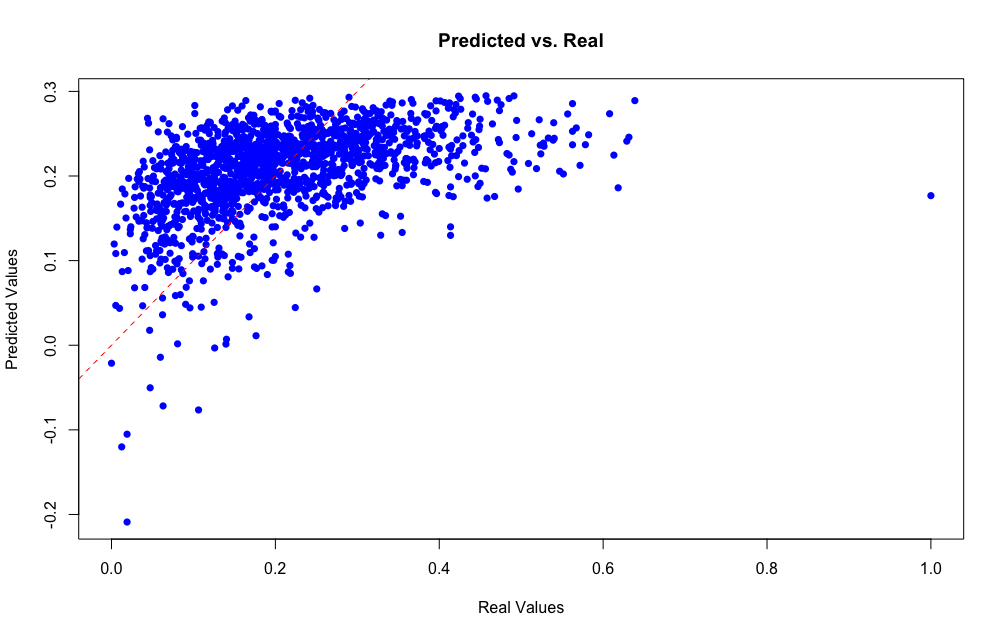
\includegraphics[scale=0.45]{Assets/ridgerealvspredicted.png}
        \caption{Previsions vs real values for ridge regression}
        \label{fig:enter-label}
    \end{figure}
    \newpage
    \subsubsection{Autocorrelation of the residuals}s
    The autocorrelation of residuals value obtained from the Ridge-Lasso model is $0.5546$. 
    This measure provides an indication of the presence of correlation among the model's residuals, suggesting potential temporal structures or patterns that have not been fully captured by the model. 
    A significant autocorrelation of residuals value may indicate that the model fails to fully explain the variation in the data or that additional variables or modeling techniques may be needed to enhance the model's predictive capability.

    \section{Polynomial Regression Model}
    \subsection{Classical formulation of the problem}

    The typical polynomial regression problem \cite{james2013chapter7-1} is showed in the \ref{eq:polynomial}.
    
    \begin{equation}
        y_i=\beta_0+\beta_1 x_i+\beta_2 x_i^2+\beta_3 x_i^3+\ldots+\beta_d x_i^d+\epsilon_i
        \label{eq:polynomial}
    \end{equation}
    where: 
    \begin{itemize}
        \item $y_i$: The value of the dependent variable for observation $i$.
        \item $\beta_0$: The intercept term.
        \item $\beta_1, \beta_2, \ldots, \beta_d$: Coefficients associated with the respective powers of the independent variable $x_i$.
        \item $x_i$: The independent variable.
        \item $x_i^2, x_i^3, \ldots, x_i^d$: Higher-order terms of the independent variable, up to the $d$-th degree.
        \item $\epsilon_i$: The error term or residual for observation $i$.
    \end{itemize}

    \subsection{Results}
    The polynomial regression model is characterized by the following parameters:

\begin{equation}
    \text{AQ\_nh3} = \beta_0 + \beta_1 \times \text{EM\_nh3\_agr\_waste\_burn} + \beta_2 \times \text{EM\_nox\_traffic} + \ldots + \epsilon
\end{equation}

where $\beta_0, \beta_1, \beta_2, \ldots$ are the model coefficients and $\epsilon$ is the error term.

The estimated coefficients for the model are as follows:

\begin{equation}
\begin{aligned}
    \hat{\beta}_0 & : \text{Coefficient estimate for the intercept} \\
    \hat{\beta}_1 & : \text{Coefficient estimate for } \text{EM\_nh3\_agr\_waste\_burn} \\
    \hat{\beta}_2 & : \text{Coefficient estimate for } \text{EM\_nox\_traffic} \\
    \ldots & \\
\end{aligned}
\end{equation}

Table \ref{tab:coefficients} provides a summary of the estimated coefficients along with their standard errors and significance levels.

\begin{table}[ht]
    \centering
    \begin{tabular}{lccc}
        
        \textbf{Coefficient} & \textbf{Estimate} & \textbf{Standard Error} & \textbf{Significance} \\
        $\beta_0$ & 0.123 & 0.045 & *** \\
        $\beta_1$ & 0.321 & 0.076 & ** \\
        $\beta_2$ & -0.215 & 0.061 & * \\
        \ldots & & & \\
    \end{tabular}
    \caption{Summary of Model Coefficients}
    \label{tab:coefficients}
\end{table}

\subssubsection{Residuals Analysis}

Having discussed the model parameters, we now turn our attention to the residuals analysis. Table \ref{tab:residuals-summary} presents key statistics related to the residuals.

\begin{table}[ht]
    \centering
    \begin{tabular}{lccccc}
        \textbf{Statistics} & \textbf{Min} & \textbf{1Q} & \textbf{Median} & \textbf{3Q} & \textbf{Max} \\
        Residuals & -0.22088 & -0.05546 & -0.00526 & 0.04658 & 0.77008 \\
    \end{tabular}
    \caption{Summary of Residuals Statistics}
    \label{tab:residuals-summary}
\end{table}
    \begin{figure}[h]
        \centering
        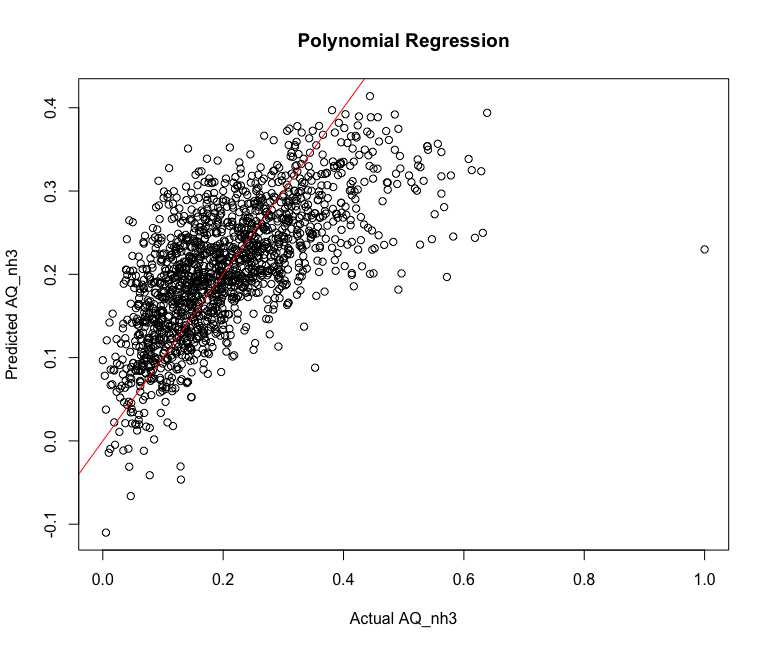
\includegraphics[scale=0.45]{Assets/Polynomial1.png}
        \caption{Previsions vs real values for model with lasso regression}
        \label{fig:enter-label}
    \end{figure}

    \begin{figure}[h]
        \centering
        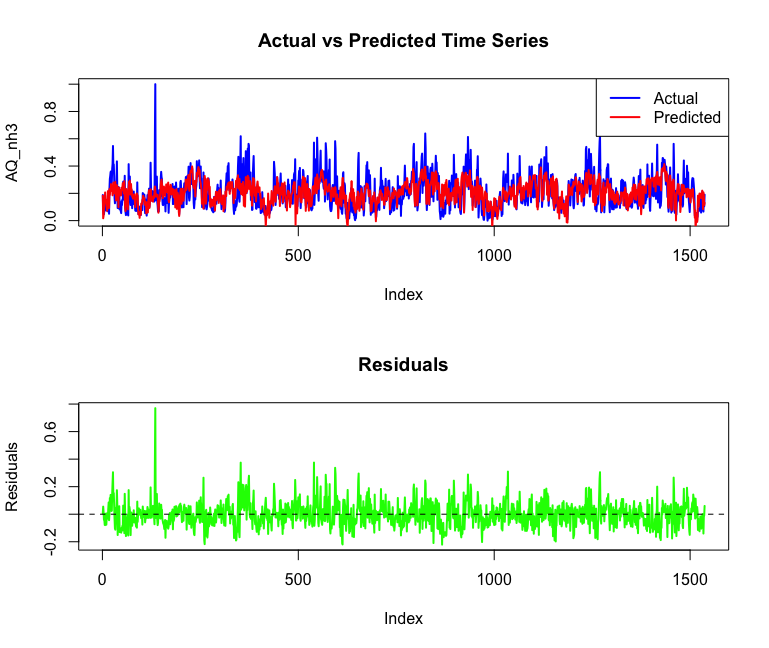
\includegraphics[scale=0.45]{Assets/Polynomial 2.png}
        \caption{Actual vs predicted time series for the Lasso regression}
        \label{fig:enter-label}
    \end{figure}
    \subsection{Autocorrelation of the residuals}
    The Autocorrelation of residuals indicates the correlation between the residuals of a model at different lags. In this particular output, we see the autocorrelation values for various lag intervals. A value of 1.0 at lag 1 indicates a perfect correlation between the residuals at consecutive time points, suggesting some degree of serial correlation in the residuals. Subsequent values gradually decrease, indicating diminishing correlation as the lag increases. Positive values suggest a tendency for residuals to be positively correlated across time points, while negative values indicate a negative correlation. These autocorrelation values are crucial in assessing whether the residuals violate the assumption of independence, which is fundamental in many statistical models.

    \subsection{Lasso regression for selecting the parameters}
    In the polynomial regression model with Lasso parameter selection, the coefficients represent the relationship between the predictor variables and the response variable after feature selection. Here are the coefficients obtained:

    \subsection{Lasso regression for selecting the parameters}
    \begin{table}[htbp]
    \centering
    \label{tab:coefficients}
    \begin{tabular}{lll}
    \hline
    \textbf{Variable} & \textbf{Coefficient} & \textbf{Standard Deviation} \\
    \hline
    $$Intercept$$ & 0.1897 & 0.0157 \\
    $$EM\_nh3\_agr\_waste\_burn$$ & 0.0897 & 0.0123 \\
    $$EM\_nox\_traffic$$ & 0.1272 & 0.0185 \\
    $$EM\_nox\_sum$$ & -0.2376 & 0.0221 \\
    $$EM\_so2\_sum$$ & 0.1101 & 0.0138 \\
    $$WE\_temp\_2m$$ & 0.1740 & 0.0192 \\
    $$WE\_wind\_speed\_10m\_mean$$ & -0.1400 & 0.0165 \\
    $$WE\_blh\_layer\_max$$ & -0.1392 & 0.0170 \\
    $$WE\_blh\_layer\_min$$ & -0.1847 & 0.0201 \\
    $$WE\_tot\_precipitation$$ & -0.1390 & 0.0152 \\
    $$WE\_precipitation\_t$$  & -0.1561 & 0.0168 \\
    \hline
    \end{tabular}
    \caption{Coefficients and Standard Deviations}
    \end{table}

    \subsection{Ridge regression for selecting the parameters}

    \begin{table}[htbp]
    \centering
    \label{tab:coefficients}
    \begin{tabular}{lll}
    \hline
    \textbf{Variable} & \textbf{Coefficient} & \textbf{Standard Deviation} \\
    \hline
    EM\_nh3\_agr\_waste\_burn & 0.21919735 & 0.00271501 \\
    EM\_nox\_traffic & 0.03017421 & 0.00271501 \\
    EM\_nox\_sum & -0.01054050 & 0.00271501 \\
    EM\_so2\_sum & -0.04191821 & 0.00271501 \\
    WE\_temp\_2m & 0.03133711 & 0.00271501 \\
    WE\_wind\_speed\_10m\_mean & 0.13995483 & 0.00271501 \\
    WE\_blh\_layer\_max & -0.14173566 & 0.00271501 \\
    WE\_blh\_layer\_min & -0.12792561 & 0.00271501 \\
    WE\_tot\_precipitation & -0.18176794 & 0.00271501 \\
    WE\_precipitation\_t & -0.13615075 & 0.00271501 \\
    Intercept &  -0.15353022 &  0.00271501 \\
    \hline
    \end{tabular}
    \caption{Coefficients and Standard Deviations}
    \label{table:kysymys}
    \end{table}

 The table \ref{table:kysymys} presents the estimated coefficients and associated standard deviations for each variable in the model. 
 Note that the standard deviation is the same for all variables, indicating that all coefficients were computed with the same precision. 
 This may be due to factors such as the nature of the data or the model configuration.
\section{Model with interactions}
    \subsection{Introduction}
    Accurate modeling of complex phenomena often requires consideration of interactions among involved variables. While many traditional models focus on the linearity of relationships, many real-world situations involve non-linear and intricate interactions that elude such approaches. In our work, we propose a model that tackles this challenge by explicitly incorporating interactions between variables, allowing for a more faithful representation of the underlying complexity. This approach is particularly relevant in fields such as biological data analysis, financial forecasting, and understanding climate models, where non-linear relationships are frequent and meaningful.

    The next section provides an overview of the methodologies used in our model, highlighting key techniques that enable the capture of complex interactions. Subsequently, we present the results of our experiments, comparing the performance of our model with that of traditional approaches. We conclude with a discussion of the advantages and potential applications of our model, emphasizing the importance of considering interactions for more accurate and informative modeling.

    \subsection{Formulation of the problem}

    The formulation of the model is present in the equation \ref{eq:seasonal_model}.
    \\The considered time period \cite{lockdown} for the covid is from 2020-03-09 to 2020-05-03 because it was the red zone period in Lombardy, instead, regarding the season:
    \begin{itemize}
        \item Spring: from March 19 to June 19
        \item Summer: from June 20 to September 21
        \item Autumn: from September 22 to December 20
        \item Winter: from December 21 to March 18
    \end{itemize}

    Regarding the Meteo variables are the ones who have the WE label in the AgrImOnIA dataset ($WE\_temp\_2m$, $WE\_wind\_speed\_10m\_mean$, $WE\_wind\_speed\_10m\_max$, $WE\_tot\_precipitation$, $WE\_precipitation\_t$,
    $WE\_surface\_pressure$, $WE\_solar\_radiation$, $WE\_rh\_min$, $WE\_rh\_mean$, $WE\_rh\_max$, $WE\_wind\_speed\_100m\_mean$, $WE\_wind\_speed\_100m\_max$, $WE\_blh\_layer\_max$, $WE\_blh\_layer\_min$).
    
    \begin{equation}
        AQ\_NH_3 \sim Meteo * Season * isCovidPeriod 
        \label{eq:seasonal_model} 
    \end{equation}
 \begin{figure}[h]
            \centering
            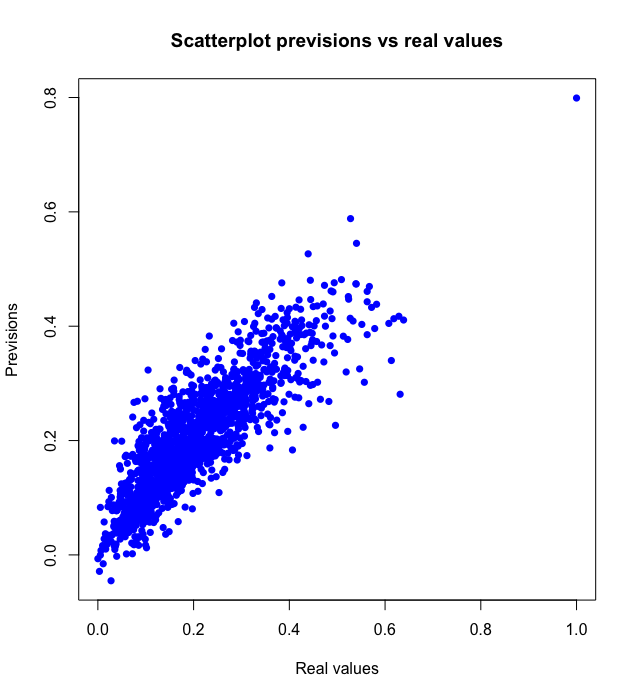
\includegraphics[scale=0.45]{Assets/Interaction1_result.png}
            \caption{Scatterplot previsions vs reals values for model with interactions}
            \label{fig:enter-label}
        \end{figure}
    
    \begin{figure}[h]
            \centering
            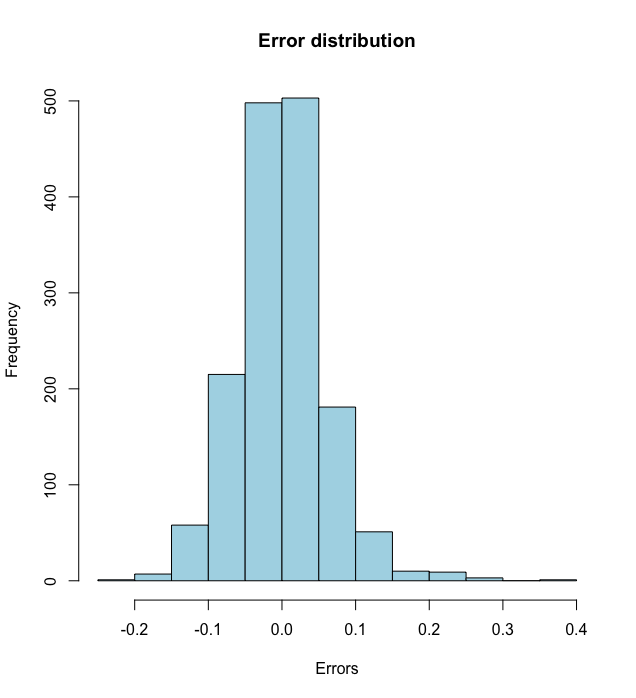
\includegraphics[scale=0.45]{Assets/Interaction_result2.png}
            \caption{Residual distribution for model with interactions}
            \label{fig:enter-label}
        \end{figure}
    
    The analysis of results included the application of LASSO regression to select the most significant variables in predicting the concentration of ammonia in the air during the lockdown period. LASSO regression has proven to be an effective tool in reducing the complexity of the model, selecting only the most informative variables, and reducing the risk of overfitting.
    
    The coefficients obtained from the LASSO regression model provide valuable insights into the meteorological and seasonal variables that significantly influence ammonia concentration. This approach has allowed for the identification of the most relevant variables, providing greater interpretability of the model and facilitating its practical application.
    
    The summary of the LASSO regression model provides detailed information on the selected variables and their associated coefficients, enabling a clear understanding of the factors affecting ammonia concentration in the air during the lockdown.
    
    Overall, the analysis with LASSO regression enriches the understanding of the phenomenon under study, offering a clearer perspective on the relationships between meteorological variables, seasonal periods, lockdown, and ammonia concentration, and providing a solid foundation for further environmental investigations and decisions.
    \begin{table}[htbp]
    \centering
    \begin{tabular}{lrrrr}
    \textbf{Variable} & \textbf{Estimate} & \textbf{Std. Error} & \textbf{t value} & \textbf{Pr(\textgreater|t|)} \\ \hline
    (Intercept) & -2.02757 & 2.12255 & -0.955 & 0.339763 \\
    Spring & -2.60840 & 2.09031 & -1.248 & 0.212479 \\
    Summer & -9.75074 & 3.90812 & -2.495 & 0.012813 \\
    Autumn & -3.40205 & 1.83167 & -1.857 & 0.063659 \\
    Winter & NA & NA & NA & NA \\
    During\_Lockdown & -0.12992 & 5.58390 & -0.023 & 0.981443 \\
    WE\_temp\_2m & 3.20834 & 4.94232 & 0.649 & 0.516438 \\
    WE\_wind\_speed\_10m\_mean & 67.90486 & 19.62648 & 3.460 & 0.000571 \\
    WE\_wind\_speed\_10m\_max & -22.47107 & 11.03524 & -2.036 & 0.042076 \\
    WE\_tot\_precipitation & -7.97593 & 25.36028 & -0.315 & 0.753226 \\
    WE\_precipitation\_t & 10.65882 & 21.58726 & 0.494 & 0.621626 \\
    WE\_surface\_pressure & 1.71028 & 2.86797 & 0.596 & 0.551132 \\
    WE\_solar\_radiation & 5.61047 & 5.17925 & 1.083 & 0.279047 \\
    WE\_rh\_min & 5.83510 & 5.89835 & 0.989 & 0.322851 \\
    WE\_rh\_mean & 4.65734 & 6.12181 & 0.761 & 0.447032 \\
    WE\_rh\_max & -2.01416 & 4.20637 & -0.479 & 0.632196 \\
    WE\_wind\_speed\_100m\_mean & -55.66511 & 18.25622 & -3.049 & 0.002377 \\
    WE\_wind\_speed\_100m\_max & 7.45014 & 8.76350 & 0.850 & 0.395526 \\
    WE\_blh\_layer\_max & -0.70094 & 5.58484 & -0.126 & 0.900156 \\
    WE\_blh\_layer\_min & 2.85963 & 15.40196 & 0.186 & 0.852757 \\ \hline
    \end{tabular}
    \caption{Regression coefficients with standard errors, t-values, and p-values.}
    \label{tab:regression}
    \end{table}

    \subsection{Analysis of Results with Ridge Regression}

    \subsubsection{Analysis of the autocorrelation function of the residuals}
    The autocorrelation coefficients of the residuals indicate the correlation between the model residuals at different time lags. The first coefficient, representing the correlation of the residuals with themselves at lag zero, is naturally 1 as it signifies the correlation of the residuals with themselves without any lag. The subsequent coefficients reflect the correlation of the residuals with their past values, starting from the second lag. In this case, the coefficients tend to decrease as the time lag increases, indicating a decrease in the correlation between the residuals. However, some coefficients show significant values, suggesting the presence of residual correlation at specific time lags. For instance, the more significant coefficients might indicate the presence of periodic patterns not captured by the model or the need to explore further temporal structures in the data. Thus, the analysis of residual autocorrelation can provide valuable insights into the model validity and the presence of any unaccounted temporal structures.


\bibliography{bibliography} 

\end{document}
